\chapter{Les peuples}

L'Empire est foulé par de nombreuses éthnies, créatures humanoïdes et intelligentes. Entre eux se tissent alors des liens, des rancunes et des amitiés... Rencontrez ces peuples durant vos aventures et qui sait, peut être en apprendrez vous plus sur leurs coutumes ?

  \section{Altmers}
  
  \begin{center}
  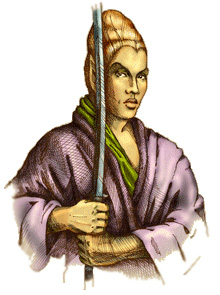
\includegraphics[width=5cm]{images/race_altmer.jpg}
  \end{center}
  
  C'est un peuple fier et arrogant, imbu de lui-même. Ils s'isolent sur l'Archipel de Summerset, et s'ils tolèrent de faire partie de l'Empire, c'est comme s'ils n'en faisaient pas partie. Il est dit que la magicka coule dans leur sang, car ce sont très souvent d'excellents mages, et le Tamriélique actuel est un dérivé de leur langue, l'Altmeri.
  
  Sveltes, fins, faibles, mais très intelligents et vifs, les altmers sont beaucoup plus souvent des mages et des politiciens que des guerriers ou des voleurs.

  \section{Argoniens}
  
  \begin{center}
  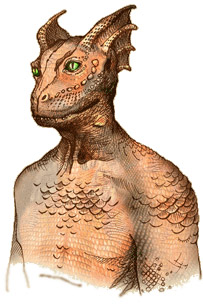
\includegraphics[width=5cm]{images/race_argonien.jpg}
  \end{center}
  
  Des humanoïdes reptiliens, peu costauds, mais très agiles et très vifs d'esprit. Les gens qui n'en ont jamais connu pensent que la lenteur de leur discours vient de leur manque d'intelligence, or il n'en est rien, la langue impériale est juste horriblement difficile à prononcer pour eux.
  
  Beaucoup font de bons mages et de bons voleurs. Certains se battent mais ce n'est pas la majorité. Enfin, certains d'entre eux sont encore esclaves, car la loi impériale n'est pas appliquée à 100\% dans toutes les provinces...

  \section{Bosmers}
  
  \begin{center}
  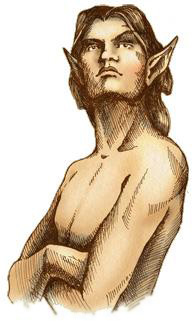
\includegraphics[width=5cm]{images/race_bosmer.jpg}
  \end{center}
  
  Comme leurs frères altmers, les bosmers sont peu costauds. Par contre, contrairement aux altmers, ils ne consacrent pas tout leur temps à acquérir des connaissances et à faire de la politique. Ce sont des gens assez proches de la nature. Ils ont appris à chasser, ont développé leurs sens, et sont parmi les meilleurs archers de Tamriel. Leur régime est principalement carnivore et des rumeurs disent dans dans certaines tribus, il y a des cannibales, des guerriers mangeant la chair des ennemis qu'ils ont tué.
  
  Récemment, l'un d'entre eux prit le pouvoir en Valenwood par la force, un Usurpateur qui devint liche, leva une armée de morts-vivants et de deadra mineurs, et marcha sur Cyrodiil. Depuis, les bosmers ne sentent coupables, par leur inaction, d'avoir laissé cette créature exister. Depuis, ils sont plutôt solitaires, et le Roi actuel a du mal à empêcher ses sujets de s'isoler où de partir en voyage hors de Valenwood.

  \section{Bretons}
  
  \begin{center}
  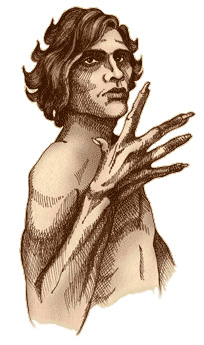
\includegraphics[width=5cm]{images/race_breton.jpg}
  \end{center}

  Bien qu'ils soient humains, car descendants des Nedes, ils semblent étrangement proches physiquement des Mers, et semblent tout aussi doués pour la magie.
  
  Ils ont aussi le défaut principal qu'ont les altmer : ils sont arrogants en général avec ceux qu'ils jugent indignes de leur respect. Heureusement, il y a des exceptions.
  
  Ce ne sont donc pas de grands combattants, mais souvent de bons marchands et d'excellents mages.

  \section{Dunmers}
  
  \begin{center}
  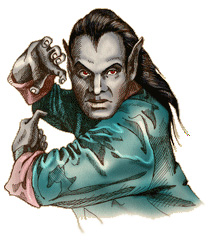
\includegraphics[width=5cm]{images/race_dunmer.jpg}
  \end{center}
  
  Il y a encore quelques siècles, les Chimers dominaient en Morrowind, leur peau ivoire légèrement dorée, semblable à celle des altmers, pouvait être jolie. Mais la colère des Aedra qui ont maudit ce peuple a causé ce noircissement leur peau.
  
  Les dunmers sont aujourd'hui couleur cendre comme leur île de Vvarfendell, les yeux rougeoyants comme la lave qui sortait jusqu'il y a peu de la montagne rouge. Ils sont assez polyvalents, car là où les altmers ont priviligié la culture et les bosmers la survie, les dunmers sont entre les deux. Ils s'essaient un peu à tout, sont très curieux. Et si un peu plus de la moitié des dunmers sont xénophobes, l'autre moitié veut commercer avec l'Empire et échanger le savoir et les connaissances, notamment les membres de la maison noble Hlaalu.

  \section{Impériaux}
  
  \begin{center}
  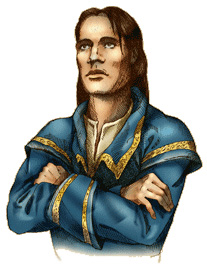
\includegraphics[width=5cm]{images/race_imperial.jpg}
  \end{center}
  
  Des dirigeants nés. Charismatiques, élégants, rusés, courageux, bien qu'ils ne soient pas particulièrement forts ou agiles, ce sont des impériaux (descendants les plus directs des Nedes, bénis par Akatosh) qui ont dirigé l'Empire pendant une bonne partie de son histoire.
  
  Ils savent diriger, gérer, mener des guerres, parlementer, et on peut avoir confiance en eux, leur notion d'honneur étant primordiale pour eux en général. Enfin ça c'est leur aspect public. En privé, qui sait...

  \section{Khajiits}
  
  \begin{center}
  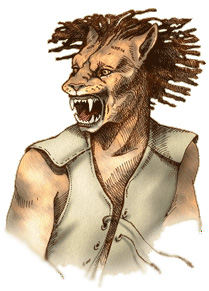
\includegraphics[width=5cm]{images/race_khajiit.jpg}
  \end{center}
  
  C'est un ensemble d'espèces humanoïdes félines réduites en esclavage pendant longtemps, certaines le sont encore. Ils sont peu intelligents, et souvent dépendants au Skooma, une drogue sucrée venant d'Elsweyr mais qui est interdite dans l'Empire. Par contre, ils sont très agiles, ont une force correcte et peuvent faire de très bons guerriers comme de bons voleurs.
  
  L'espèce que l'on peut croiser en Tamriel est la plus courante, celle qui ressemble le plus à un humain, hormis la tête, les pattes, et la pilosité.

  \section{Nordiques}

  \begin{center}
  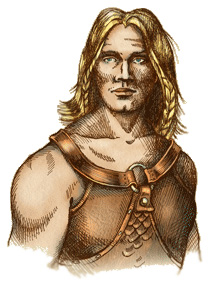
\includegraphics[width=5cm]{images/race_nordique.jpg}
  \end{center}
  
  De fiers et solides gens que les nordiques ! En bravant continuellement le froid, en faisant de la valeur au combat un facteur d'échelle sociale, c'est le peuple qui a le plus de véritables maîtres du combat. Des tatouages se voient souvent sur eux, car leurs croyances impliquent des protections contre le mauvais œil, afin que rien ne vienne gâcher leurs combats.
  
  Ils sont cependant agréables et courtois, bien qu'un peu rudes.

  \section{Orsimers}

  \begin{center}
  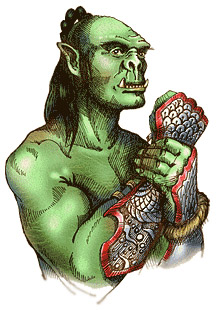
\includegraphics[width=5cm]{images/race_orsimer.jpg}
  \end{center}
  
  Pendant longtemps, les Orsimers ont été exterminés, étant vus comme des monstres sans cervelle. Mais quand l'Usurpateur-liche de Valenwood attaqua Cyrodiil, les Orsimers y virent un moyen de prouver leur intelligence, en aidant les troupes impériales à défendre l'Empire. Cela n'a pas marché tout de suite, mais les Orsimers ont fini par avoir leur cité-état Orsinium, et y vivent en majorité aujourd'hui.
  
  Ils sont forts, rudes, peu dextres, mais ce sont les meilleurs forgerons de l'Empire, de peu devant les artisans nordiques.
  
  Des mythes expliquent que les Orsimers seraient des Chimers maudits d'une autre manière que les Dunmers n'étant pas en Morrowind à ce moment-là, ayant pris la fuite.

  \section{Rougegardes}

  \begin{center}
  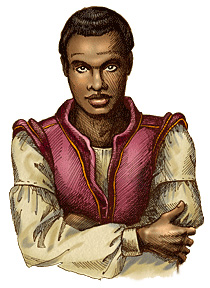
\includegraphics[width=5cm]{images/race_rougegarde.jpg}
  \end{center}
  
  Encore un peuple de guerriers arrogants, de peau sombre, mais d'une loyauté sans faille.
  
  Les rougegardes sont des combattants émérites, maîtres de l'art du combat, séducteurs mais avec une notion de l'honneur encore plus pointue que les impériaux.
  
  Les combattants rougegardes les plus âgés sont souvent d'excellents maîtres d'armes.

